\documentclass{beamer}
% \usetheme{Warsaw}

\usefonttheme[onlymath]{serif}

\setbeamertemplate{caption}[numbered]
\setbeamertemplate{bibliography item}{\insertbiblabel}

\addtobeamertemplate{navigation symbols}{}{%
    \usebeamerfont{footline}%
    \usebeamercolor[fg]{normal text}%
    \hspace{1em}%
    \insertpagenumber
}

\definecolor{Primary}{RGB}{0,0,0}
\definecolor{Secondary}{RGB}{154, 32, 140} \definecolor{Thirdary}{RGB}{225, 18, 153}

\setbeamercolor{structure}{fg=Secondary}
\setbeamercolor{normal text}{fg=Primary}
\setbeamercolor{alerted text}{fg=Thirdary}

% language
\usepackage[T2A, T1]{fontenc}
\usepackage[utf8]{inputenc}
\usepackage[russian]{babel}

% % language
% \usepackage{fontspec}
% \usepackage{polyglossia}
% \usepackage[norwegian=guillemets]{csquotes}
% \setmainfont{Times New Roman}
% \setmonofont{DejaVu Sans Mono}
% 
% \setdefaultlanguage{russian}
% \setotherlanguage{english}
% 
% % \defaultfontfeatures{Ligatures = TeX}
% % 
% % \setmainlanguage[babelshorthands=true]{russian} 
%  
% \setmainfont{cmun}[
%   Extension=.otf,
%   UprightFont=*rm,
%   ItalicFont=*ti,
%   BoldFont=*bx,
%   BoldItalicFont=*bi,
%   SlantedFont=*sl,]
% 
% \setsansfont{cmun}[
%   Extension=.otf,
%   UprightFont=*ss,
%   ItalicFont=*si,
%   BoldFont=*sx,
%   BoldItalicFont=*so,]
% 
% \setmonofont{cmun}[
%   Extension=.otf,
%   UprightFont=*btl,% light version
%   ItalicFont=*bto,%  light version
%   BoldFont=*tb,
%   BoldItalicFont=*tx,
% ]

\usepackage{graphicx}
\usepackage{multicol}

% \bibliographystyle{gost-numeric}
% \usepackage[
%     style=gost-numeric,
%     citestyle=numeric
% ]{biblatex}
% \addbibresource{refs.bib}

\title{Кластеризация пациентов по генам}
\author{Костеров М. А.}
\date{}

\newcommand\R{\mathbb{R}}

\newcommand\parallelitem[2]{
    \begin{columns}[t]
        \begin{column}{0.5\textwidth}
            \begin{itemize}
                \item{} #1
            \end{itemize}
        \end{column}
        \begin{column}{0.5\textwidth}
            \begin{itemize}
                \item{} #2
            \end{itemize}
        \end{column}
    \end{columns}
}

\begin{document}

\begin{frame}
  \titlepage
\end{frame}

\begin{frame}{Задача}
  \begin{figure}
    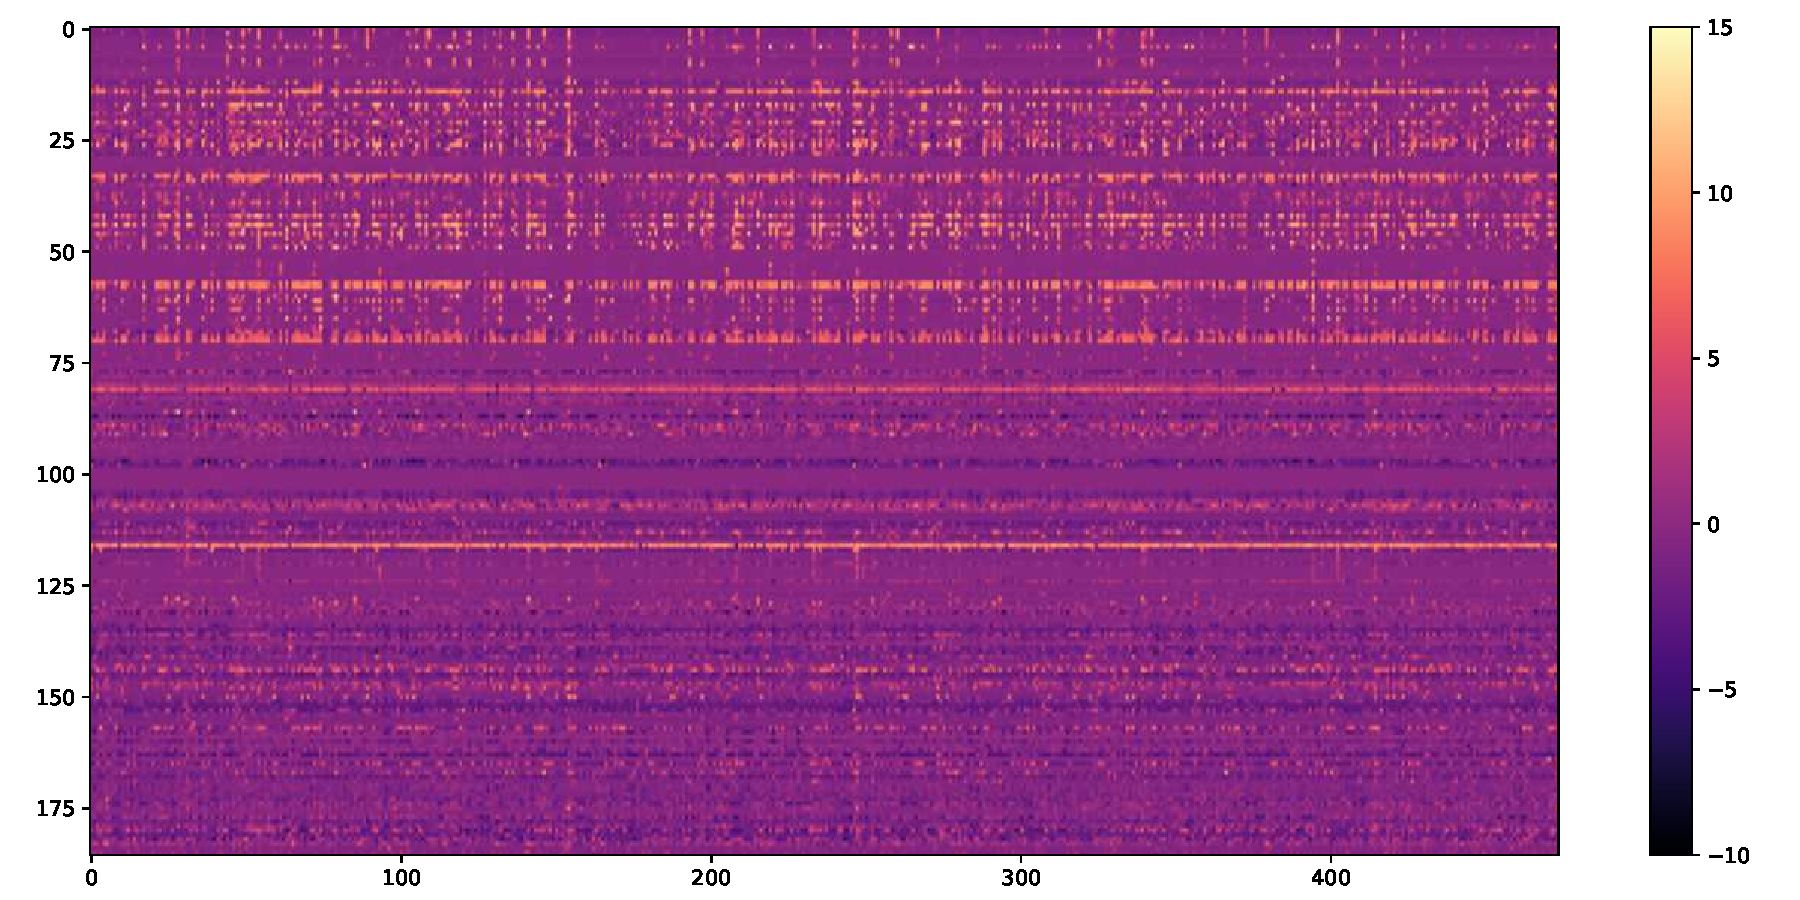
\includegraphics[width=1.0\textwidth]{./figures/full_genes.pdf}

    \caption{Выраженность генов у пациентов. Пациенты по $x$, гены по $y$.}
  \end{figure}

  {\bf Задача.} Кластеризовать пациентов по генам, автоматически определяя
  число кластеров. Задача может возникать в исследованиях взаимосвязи риска
  рака и генов.
\end{frame}

\begin{frame}{Методы. Аппроксимационно-оценочные критерии}
  \begin{overprint}
    \onslide<1>
    \begin{figure}
      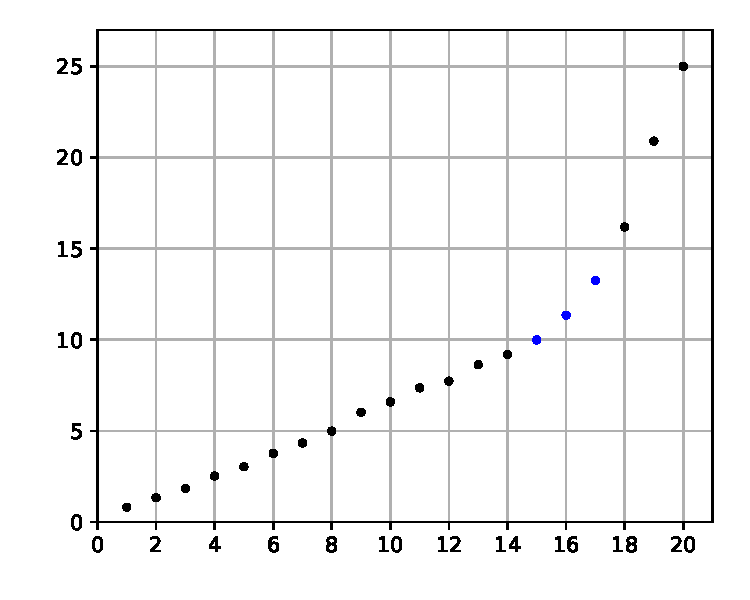
\includegraphics[width=0.7\textwidth]{./figures/elbow.pdf}

      \caption{Некоторая последовательность. В выделенных синим точках ее рост
        переходит от линейного к нелинейному.}
    \end{figure}

    \onslide<2>
    \begin{figure}
      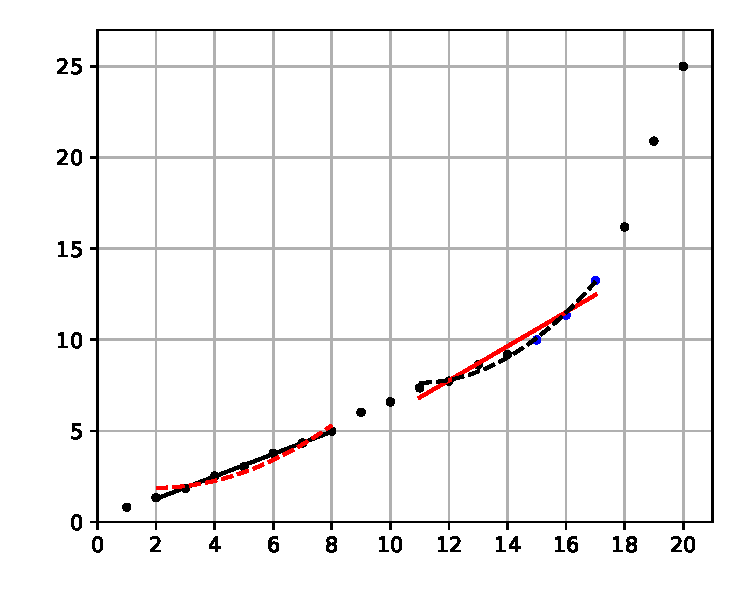
\includegraphics[width=0.7\textwidth]{./figures/elbow-parabolic.pdf}

      \caption{Формально этот локоть можно определить с помощью приближения
        функциями $at+b$ и $at^{2}+b$ соответственно. Окно 2--8 лучше
        приближается линейной функцией, окно 11--17~--- уже нелинейной.
      }
    \end{figure}
  \end{overprint}
\end{frame}


\begin{frame}{Методы. Аппроксимационно-оценочные критерии}
  Определяя формально, зафиксируем размер окна $k$ и последовательность
  $\{y_{i}\}_{i=1}^{N}$. Будем рассматривать окна вида
  \[
    y_{k_0-k+1},y_{k_0-k+2},...,y_{k_0}.
  \]
  \[
    \delta^{2}_{l}(k_0):=\min_{a,b}\sum_{i=1}^{k}(ai+b-y_{k_0-k+i})^{2},
  \]
  \[
    \delta^{2}_{f}(k_0):=\min_{a,b}\sum_{i=1}^{k}(a(i-1)^{2}+b-y_{i})^{2},
  \]
  \[
    \delta^{2}(k_0):=\delta_{f}(k_0)-\delta_{l}(k_0),
    \quad
    t_0:=\min\{k_0\geq k~|~\delta^{2}(k_0)>0\}.
  \]
  Согласно параболическим аппроксимационно-оценочным критериям, локоть
  находится между $t_0-1$ и $t_0$. До $t_0-1$ включительно рост был линейный.
  Если множество под минимумом пустое, будем считать, что $k_0=N$.
\end{frame}

\begin{frame}{Методы. Агломеративная кластеризация}
  Агломеративная кластеризация начинает с определения каждого элемента выборки
  $\mathcal X=\{X_{i}\}_{i=1}^{N}$ в свой единичный кластер, после чего на
  каждом шаге два некоторых кластера объединяют. Выбор двух кластеров
  проводят по некоторому критерию.

  \vfill

  Используемый в данной работе метод (метод Варда, Ward's method) минимизирует
  рост внутрикластерного суммарного квадратичного отклонения. На шаге $k$ его
  определяют как
  \[
    d^{(k)} := \sum_{i=1}^{M^{(k)}}\sum_{j=1}^{N^{(k)}_{i}}\left(Y^{(k)}_{i,j} - \mu_{i}\right)^{2},\quad
    \mu^{(k)}_{i}:=\frac{1}{N^{(k)}_{i}}\sum_{j=1}^{N^{(k)}_{i}}Y^{(k)}_{i,j},
  \]
  где $\mathcal C^{(k)}_{i}=\{Y^{(k)}_{i,j}\}_{j=1}^{N^{(k)}_{i}}$~--- кластер,
  $M^{(k)}$~--- число кластеров. $\{\mathcal
    C^{(k)}_{i}\}_{i=1}^{M^{(k)}}$~--- разбиение $\mathcal X$.
\end{frame}

\begin{frame}{Методы. Локоть в последовательности минимальных расстояний}
  Рассмотрим последовательность
  \[
    F_{k}:=\min_{\substack{1\leq i,j\leq M^{(k)}\\ i\neq j}}
    \min_{\substack{Z_1\in\mathcal C^{(k)}_{i},\\ Z_2\in\mathcal C^{(k)}_{j}}}
    ||Z_1-Z_2||_{2}
  \]
  минимальных расстояний между кластерами. Для метода Варда она монотонно возрастающая.

\end{frame}

\begin{frame}{Методы. Локоть в последовательности минимальных расстояний}
  На искусственном примере, намеренно сгенерированным таким образом, что
  можно кластеризовать на $5$ и $25$ кластеров видны локти последовательности
  минимальных расстояний.

  \begin{overprint}
    \onslide<1>
    \begin{figure}
      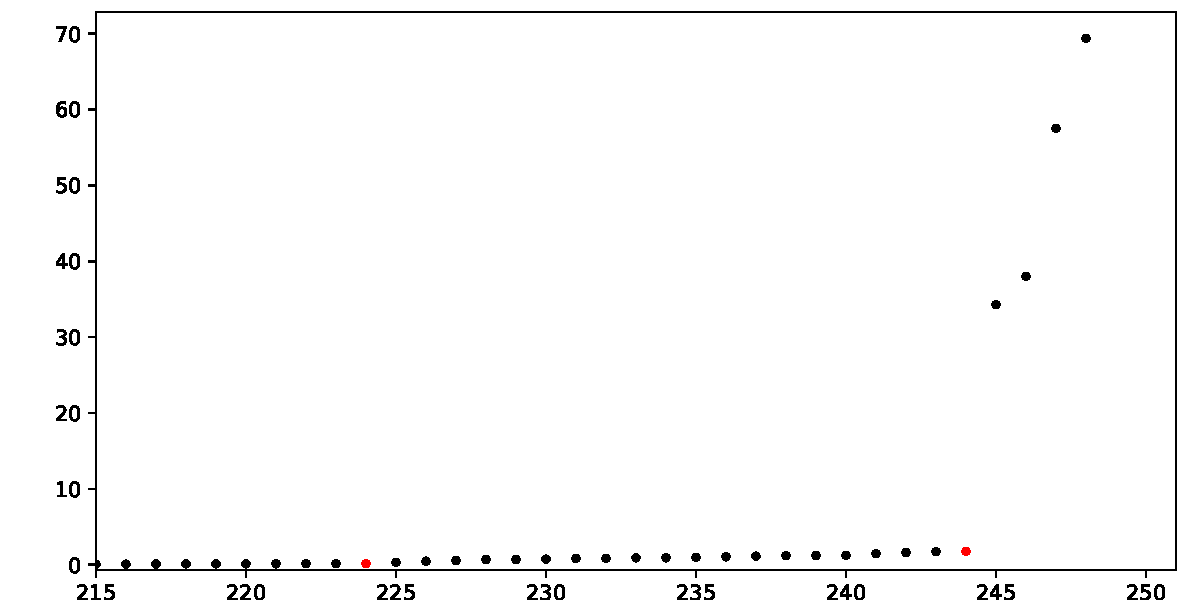
\includegraphics[width=0.9\textwidth]{./figures/agglomerative-elbow-1.pdf}

      \caption{Локоть последовательности минимальных расстояний для $5$ кластеров.}
    \end{figure}

    \onslide<2>
    \begin{figure}
      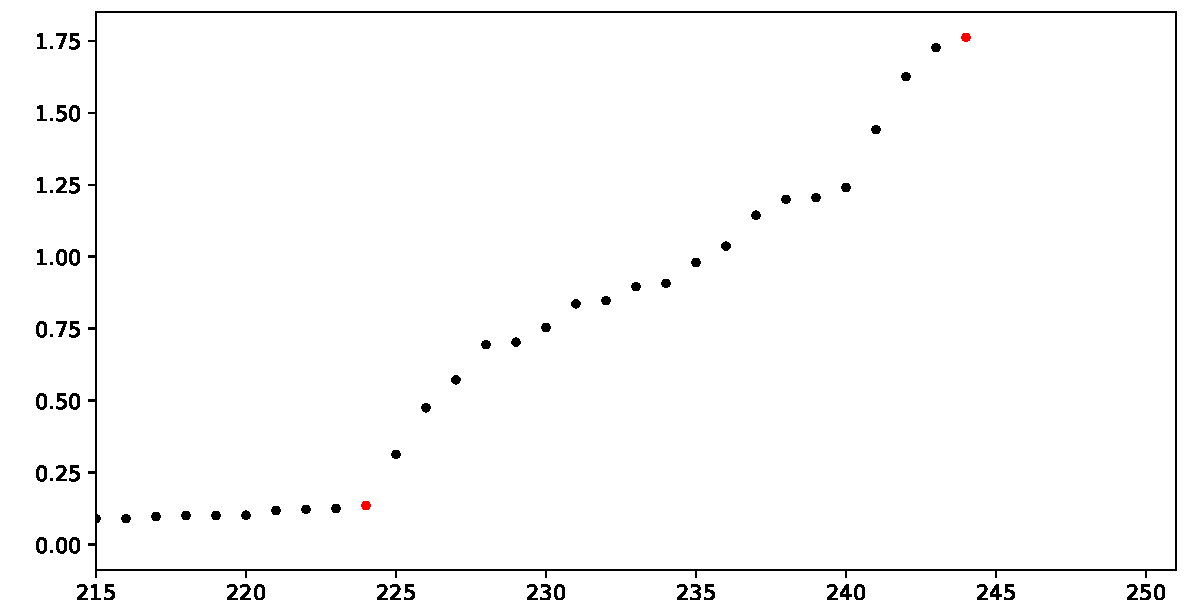
\includegraphics[width=0.9\textwidth]{./figures/agglomerative-elbow-2.pdf}

      \caption{Локоть последовательности минимальных расстояний для $25$ кластеров.}
    \end{figure}
  \end{overprint}
\end{frame}

\begin{frame}{Методы. Выбор реккомендованного числа кластеров}
  \vfill

  При анализе вместо $F_{k}$ рассматривают последовательность
  $y_{k}(p)=F_{k}+pk$, где $p>0$. Добавку $pk$ называют линией тренда. Пусть
  $k_0(p)$ --- локоть последовательности $y_{k}(p)$ согласно параболическому
  аппроксимационно-оценочному критерию.

  \vfill

  Определим $M(p):=N-k_0(p)$ --- число кластеров при определенном $p$.

  \vfill

  Зафиксируем $k$ и будем рекомендовать наиболее <<устойчивые>> числа кластеров
  большие некоторого минимума $M_{\min}$. Устойчивость числа кластеров $M_0$
  определяется как наибольшая длина отрезка $[p_0,p_1]$, в котором
  $M(p)=M_0$.

  \vfill
\end{frame}

\begin{frame}{Методы. Выбор реккомендованного числа кластеров}
  \begin{figure}
    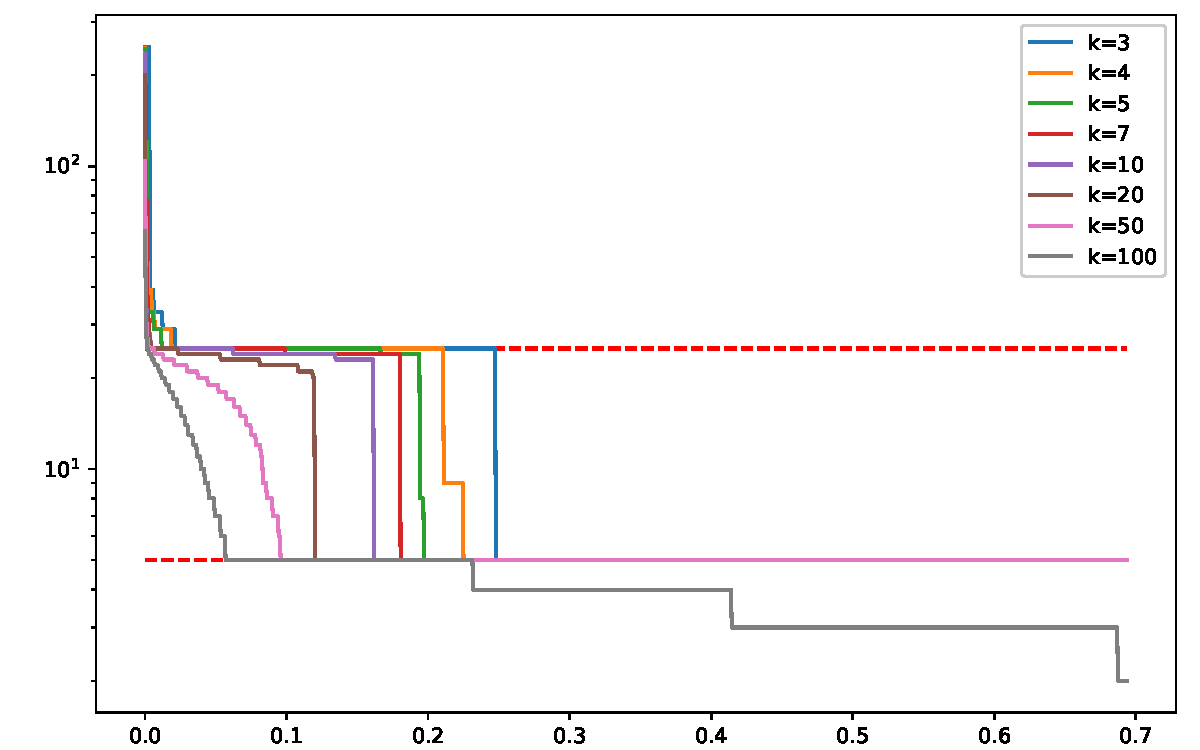
\includegraphics[width=1.0\textwidth]{./figures/trend-analysis.pdf}

    \caption{Зависимость $M(p)$ от $p$ и $k$ в случае искусственного примера.}
  \end{figure}
\end{frame}

\begin{frame}{Результаты}
  В реализации были выбраны параметры $k=4$ и $M_{\min}=5$.

  \begin{figure}
    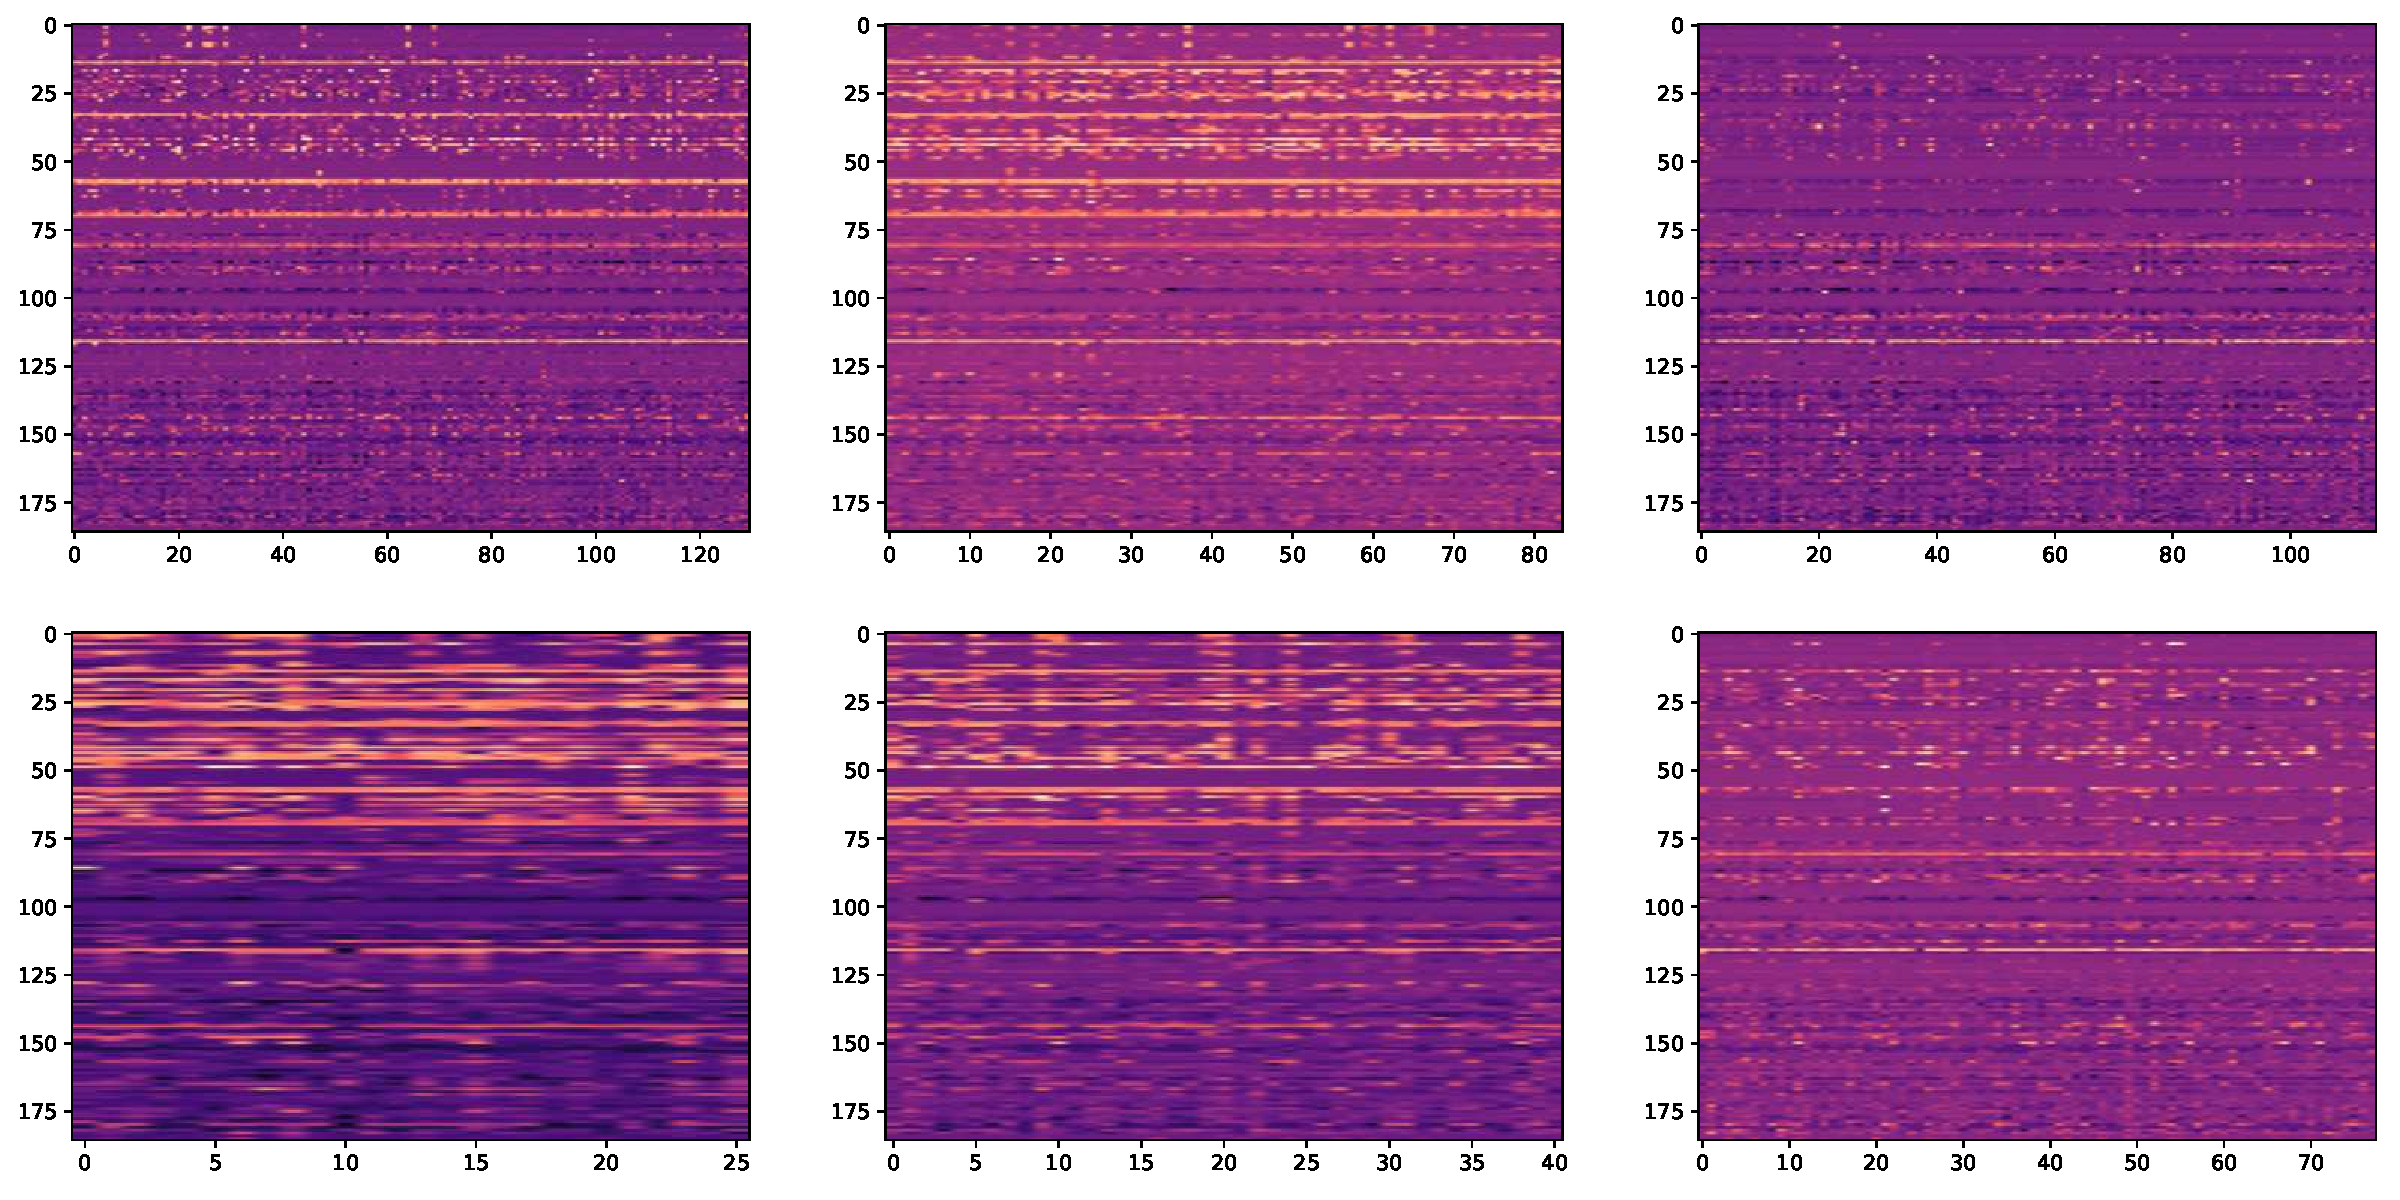
\includegraphics[width=1.0\textwidth]{./figures/result.pdf}

    \caption{Один из примеров предложенной кластеризации. Длина отрезка $p$
      равна $8.15$.}
  \end{figure}
\end{frame}

\end{document}
